\chapter{Electron-Ion Collider}\label{cha:EIC} % chktex 24

The Electron-Ion Collider (EIC) is a planned accelerator facility to be built at Brookhaven National Laboratory [cite BNL] in the place of today's Relativistic Heavy Ion Collider (known as RHIC). Contrary to RHIC, which was built as an ion-ion collider, EIC will open new possibilities of probing the structure of nucleons by colliding the more complicated ions  with the comparably "simple-structured" electrons. Its versatile design will allow for the usage of a wide range of these ions: from protons (hydrogen ions) up to ions of uranium [cite Silvia DIS].

The key scientific questions to be addressed by the EIC will be integrated into the final design of the whole accelerator complex, as well as of every experiment and its detectors within. One of these is investigating fundamental properties of nucleons, such as their mass and spin, and discovering how they emerge from the interactions of the partons (gluons and quarks) they are made of. Speaking of the partons, another puzzle for the EIC is to solve how they are distributed inside nucleons, both in momentum and in position. It is also of high interest to discover how they interact with a nuclear medium, what makes the confined hadronic states emerge from these partons, and if the density of gluons keeps growing with increasing energies or if it reaches a point of saturation [cite YR].

In order to solve these conundrums, there are some performance requirements imposed on the design of the EIC. Among them is the large range and variability of center of mass energies, which should range from approximately 20 GeV, up to 100 GeV with a future possibility of reaching 140 GeV. This is needed in order to effectively map out the nuclear structure through various scales of Bjorken $x$. Next, th EIC will boast extraordinarily high luminosity of up to $10^{34}$~cm$^{-2}$\,sec$^{-1}$ in order to gain access to rare probes and rare events [cite LRP2015]. The peak luminosities for different combinations of electron and proton energy are shown in Figure~\ref{fig:eic:lumi}. Compared to its spiritual predecessor (that is the collider HERA\footnote{HERA (or \emph{Hadron-Elektron Ring Anlage} in German) was an electron-proton collider in the DESY laboratory in Hamburg, Germany. It operated between the years 1997 and 2007 [cite HERA].}), which reached a peak luminosity of $5 \cdot 10^{-31}$~cm$^{-2}$\,sec$^{-1}$~[cite HERA], the EIC is designed to achieve luminosity roughly three orders of magnitude greater. Lastly, there needs to be a open possibility for a second (complementary) detector, which would provide an independent confirmation for discovery measurements and an overall expansion of scientific opportunities [cite source2].

\section{From RHIC to EIC}
For more than twenty years RHIC has been a cornerstone of nuclear and particle physics. Commissioned in 2000, it was the first collider able to collide ions heavier than protons, creating the hot, dense conditions akin to those of the early universe [cite RHIC-facts]. It was built as the result of a compromise between particle physicists interested in the mechanism of multi-particle production in high-energy hadron collisions and nuclear physicists interested in investigating the nuclear equation of state with the highly compressed nuclear matter. RHIC also pioneered the use of spin-polarized proton beams [cite RHIC-program].

The legacy of innovation continues with the EIC, which will also incorporate a polarized electron beam into its design. The EIC, shown in Figure~\ref{fig:eic:eic}, will reuse much of the existing RHIC infrastructure, some of which are: the tunnel, the "Yellow" Ring (shown in Figure~\ref{fig:eic:rhic}), cryogenic systems, some of the magnets, and more. The main changes will involve adding a new electron accelerator and modifying the existing ion accelerator to accommodate electron-ion collisions [cite CDR]. This approach significantly reduces costs, while it also leverages the proven capabilities of RHIC.

\begin{figure}[ht]
    \centering
    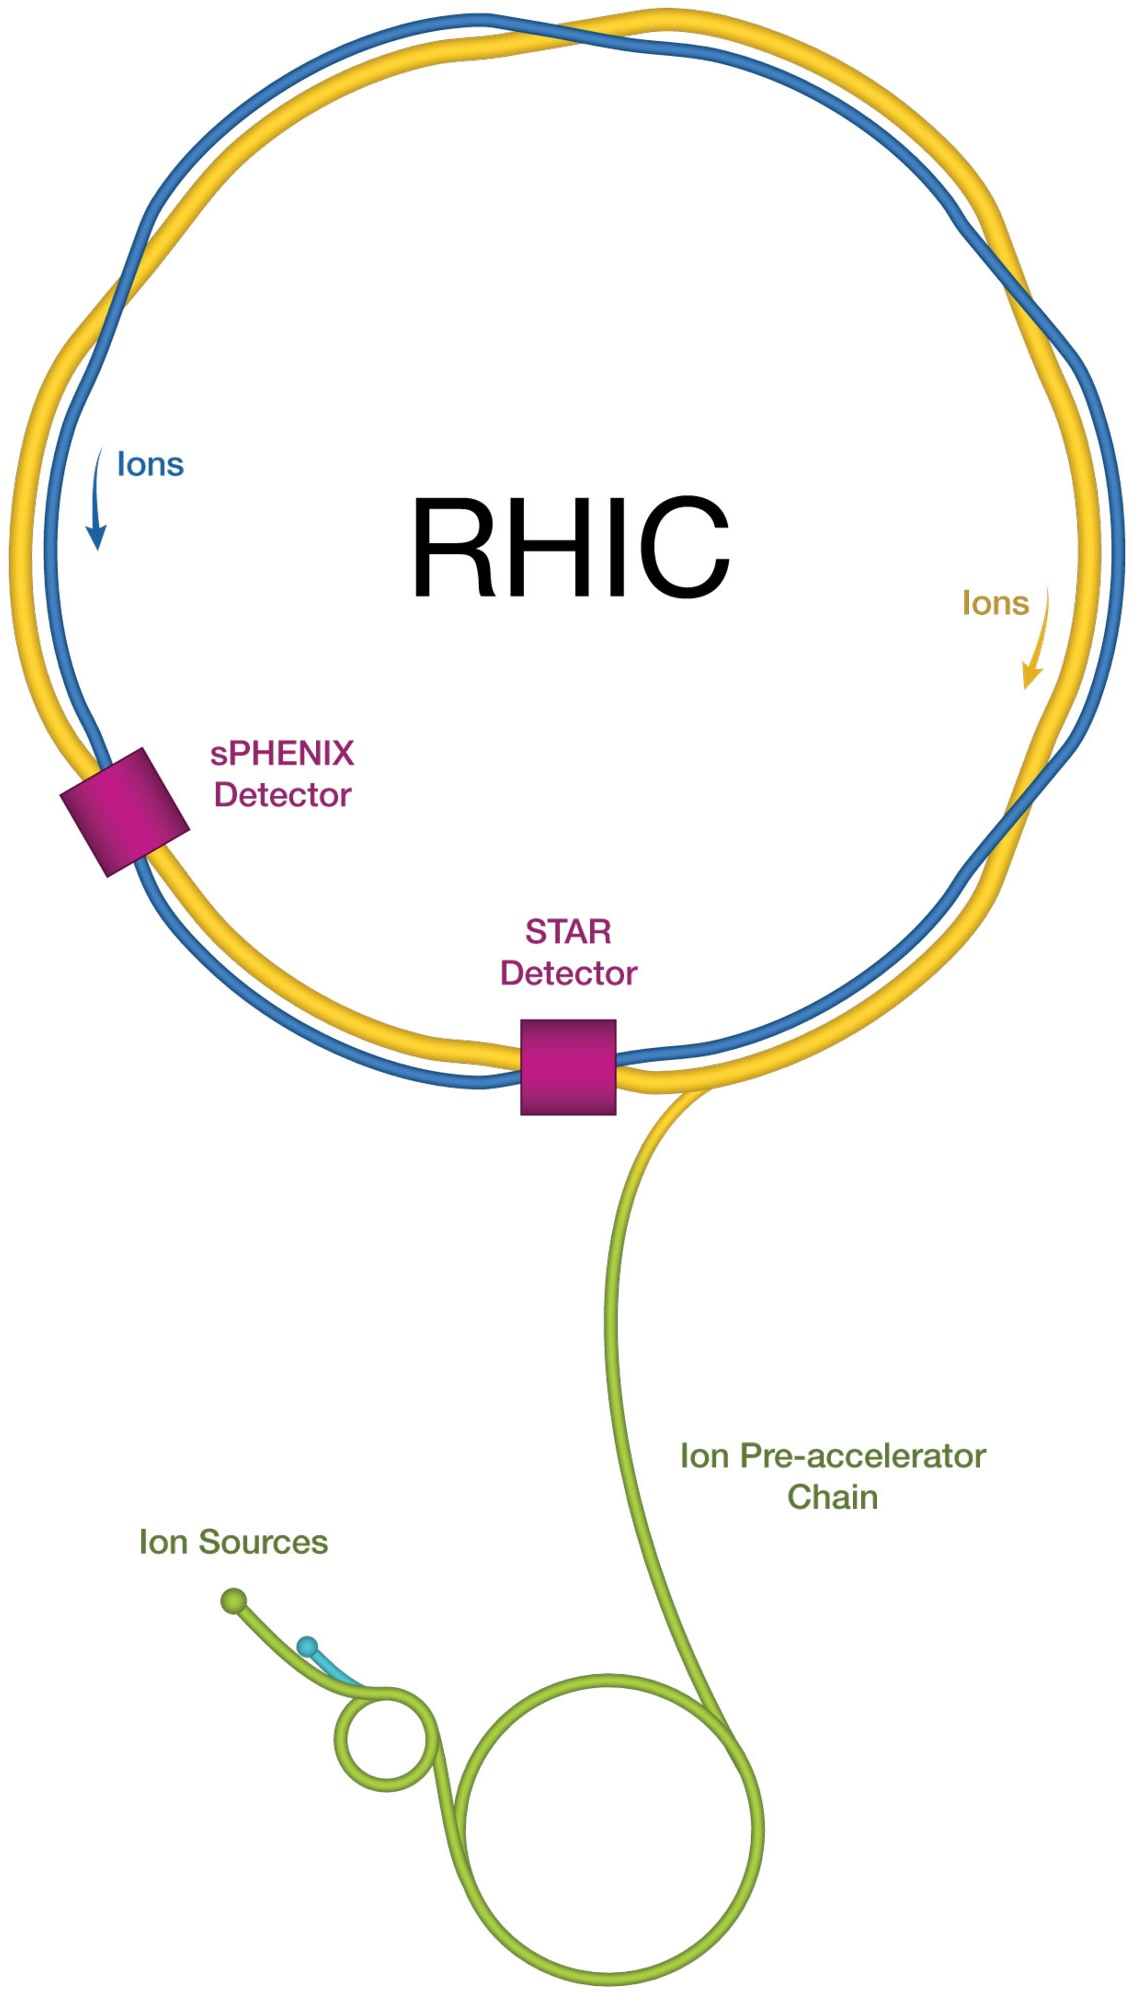
\includegraphics[width=.3\linewidth]{img/rhic.jpg}
    \caption{Layout of the existing RHIC facility. The "Yellow" Ring planned for reuse in the EIC is shown in yellow. Taken from [cite RHIC image].}
    \label{fig:eic:rhic}
\end{figure}

\begin{figure}[ht]
    \centering
    \includegraphics[width=.8\linewidth]{img/EIC_new.png}
    \caption{Current design of the EIC. Taken from [cite EIC-new-image].}
    \label{fig:eic:eic}
\end{figure}

\begin{figure}[ht]
    \centering
    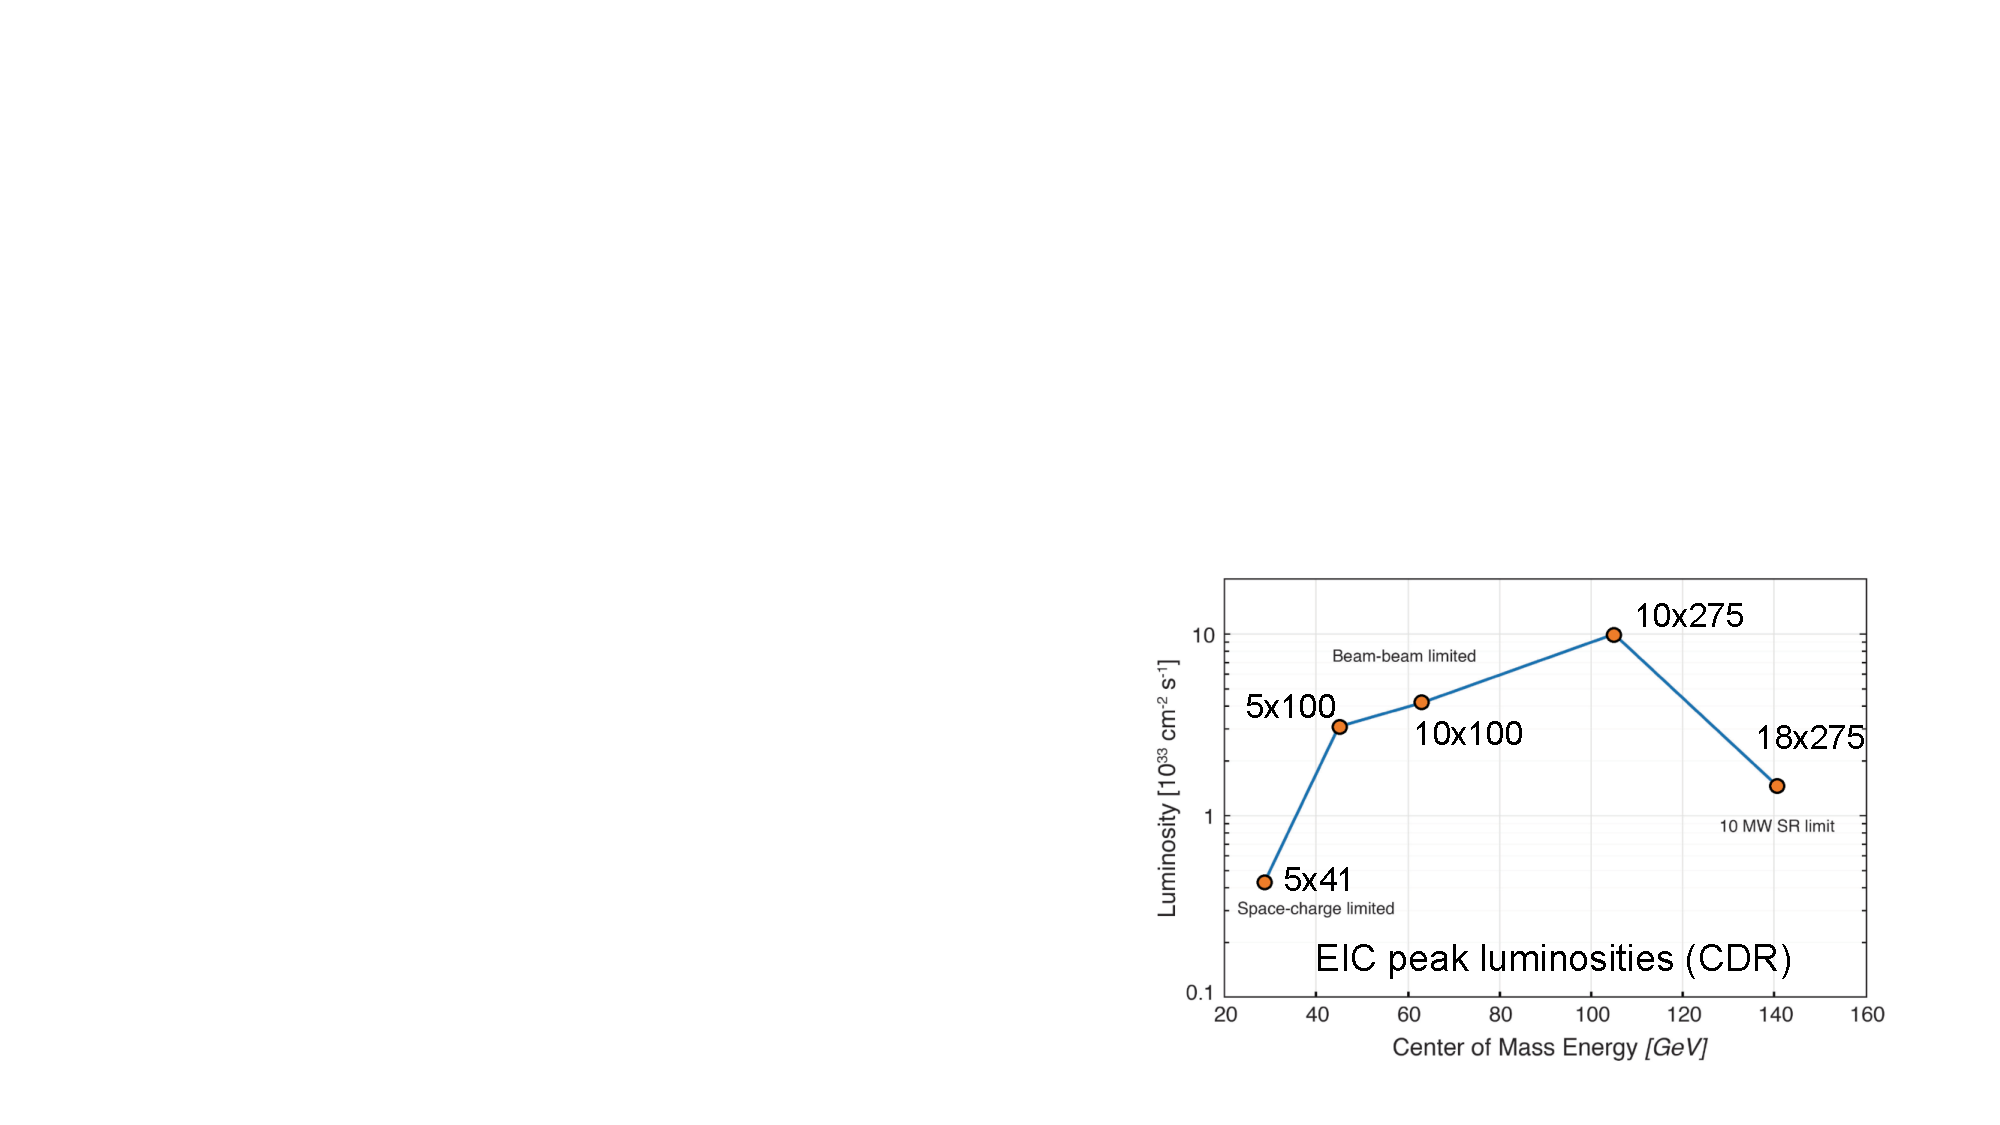
\includegraphics[width=.7\linewidth]{img/luminosity2_placeholder.pdf}
    \caption{PLACEHOLDER Peak luminosities for different electron$\times$ion energy combinations. Taken from [cite MOA1].} % aj v eic_cdr_final.pdf na s. 18
    \label{fig:eic:lumi}
\end{figure}


\section{Hadrons}
The hadronic component of the EIC will greatly benefit from the reused infrastructure of RHIC. Recalling again the connection with HERA, which was limited to electron-proton collisions, the EIC will accommodate a wide variety of heavier ions. These hadron beams, at least those made of protons and light nuclei (such as \isotope[3]{He}), will be highly polarized, reaching up to 70\% [cite LRP2015].

\subsection{Particle sources}
Following in the steps of RHIC, the EIC will also utilize a polarized hadron beam. This lends an opportunity to reuse the currently existing infrastructure, especially for creating and accelerating polarized protons. 

Production of negatively charged hydrogen ions in RHIC is handled by the Optically Pumped Polarized Ion Source (OPPIS), which has been in use since the beginning of RHIC's program and during its lifetime has gone through several upgrades. [cite polA-sources] Polarization in the OPPIS is achieved with a circularly polarized laser beam, which is used to polarize an atom of rubidium. Meanwhile a hydrogen atom is ionized by an atom of helium. The now ionized hydrogen atom (that is, a proton) captures a polarized electron from the atom of rubidium. The polarization is then transferred from the electron to the proton. At the end of this process, the polarized, but electrically neutral, hydrogen atom has to capture a second electron, so it may be then accelerated. [cite polP-EIC]

In order to fulfill the scientific plan, there is a strong need and demand for a beam of polarized neutrons. Unfortunately, as is evident, neutrons by themselves cannot be accelerated. It is necessary to resort to some charged ion that would contain the desired neutrons. The first logical step from a lone neutron would be some ion of deuterium, which contains an additional proton. A feasibility study has already been done for acceleration of polarized deuterons in the EIC, which deemed it possible [cite deuteron-feasibility]. However, the small magnetic moment of deuterium could pose a challenge for spin manipulation. That makes helions (\isotope[3]{He}) a preferred alternative, as the most abundant state of \isotope[3]{He} has the protons' spins anti-aligned, which makes the neutron practically carry the nuclear spin. Therefore, helions make for an effective spin-polarized neutron source [cite EIC-scientific-beams]. They are to be produced in the Electron Beam Ion Source (EBIS), which will also remain the particle source of choice for heavier ions for the EIC [cite optically-pumped]. Possibility of extending the polarization to heavier ions, such as \isotope[6]{Li} or \isotope[7]{Li}, is still under discussion, as it could prove beneficial for gaining new insights into quark-gluon dynamics within the nuclear medium, or even beyond [cite scientific-beams]. 

\subsection{Preacceleration}
Before entering the EIC's Hadron Storage Ring (HSR), the beam needs to undergo several steps of preacceleration. This infrastructure is to be inherited from the initial acceleration systems used by RHIC. Travelling through it, protons coming from a source get first accelerated in a Linear Accelerator (LINAC) to energy of 200 MeV, then pass through a booster synchrotron (known as Booster) with energy of 1.5 GeV, and lastly they enter the Alternating Gradient Synchrotron (AGS), from which they come out with energy of 25 GeV [cite Nagaitsev Frascati]. All of the aforementioned accelerators are shown in Figure~\ref{fig:eic:eic}.

\subsection{Hadron Storage Ring}
The reuse of the arcs of at least one of RHIC's storage rings has been a part of the design plan of the EIC since the beginning [cite CDR]. Ultimately, after assessing the tunnel and considering the requirements for accessibility, the “Yellow” ring was chosen to be kept in its entirety. Its existing arcs will live on as the HSR after removal of a number of magnets from Interaction Region 6 (IR6) and from Interaction Region 2 (IR2), due to significant modifications in these regions [cite EIC-design-highlights]. Because the EIC will use a much larger number of bunches of shorter length than RHIC, resulting in the beam current being increased by a factor of 3 [cite RHIC-to-EIC-HSR], new actively cooled beam screens will be inserted into the superconducting magnet beam pipes. These sleeves will be coated with copper to reduce electric resistivity and with a secondary layer of amorphous carbon to prevent the accumulation of electron clouds [cite scientific-beams]. 

In order to preserve polarization of the beam, there are already two Siberian snakes\footnote{Siberian snakes are devices that rotate the spin vectors of the beam particles by \ang{180} each turn, in order to mitigate the effect of depolarizing resonances in circular accelerators [cite siberian-snakes].} present in RHIC. Additional four will be installed in the HSR - two of those coming directly from the RHIC's "Blue" ring, and two will be built from spin rotators from the same ring [cite scientific-beams].

%cooling :((

\section{Electrons}
Comparable to the hadron beam, also the energy of the electron beam is required to be variable. The chosen beam energies are 5 GeV, 10 GeV, and 18 GeV. In another parallel with the hadron beam, the electron beam must reach the same high levels of average polarization, that is 70\% [cite LRP2015]. 

HERA polarized by Sokolov-Ternov, EIC polarized from the source [Nagaitsev:MOA1]

\subsection{RCS (or Pre-acceleration)}


A beam-accumulator-ring (BAR) is then used to provide 7 nC or 28 nC bunches (depending on final beam energy) to the Rapid Cycling Synchrotron (RCS) [cite EIC-scientific-beams]. 

\subsection{Electron Storage Ring}

\section{Interaction Region 6 (IR6)}

\begin{figure}[ht]
    \centering
    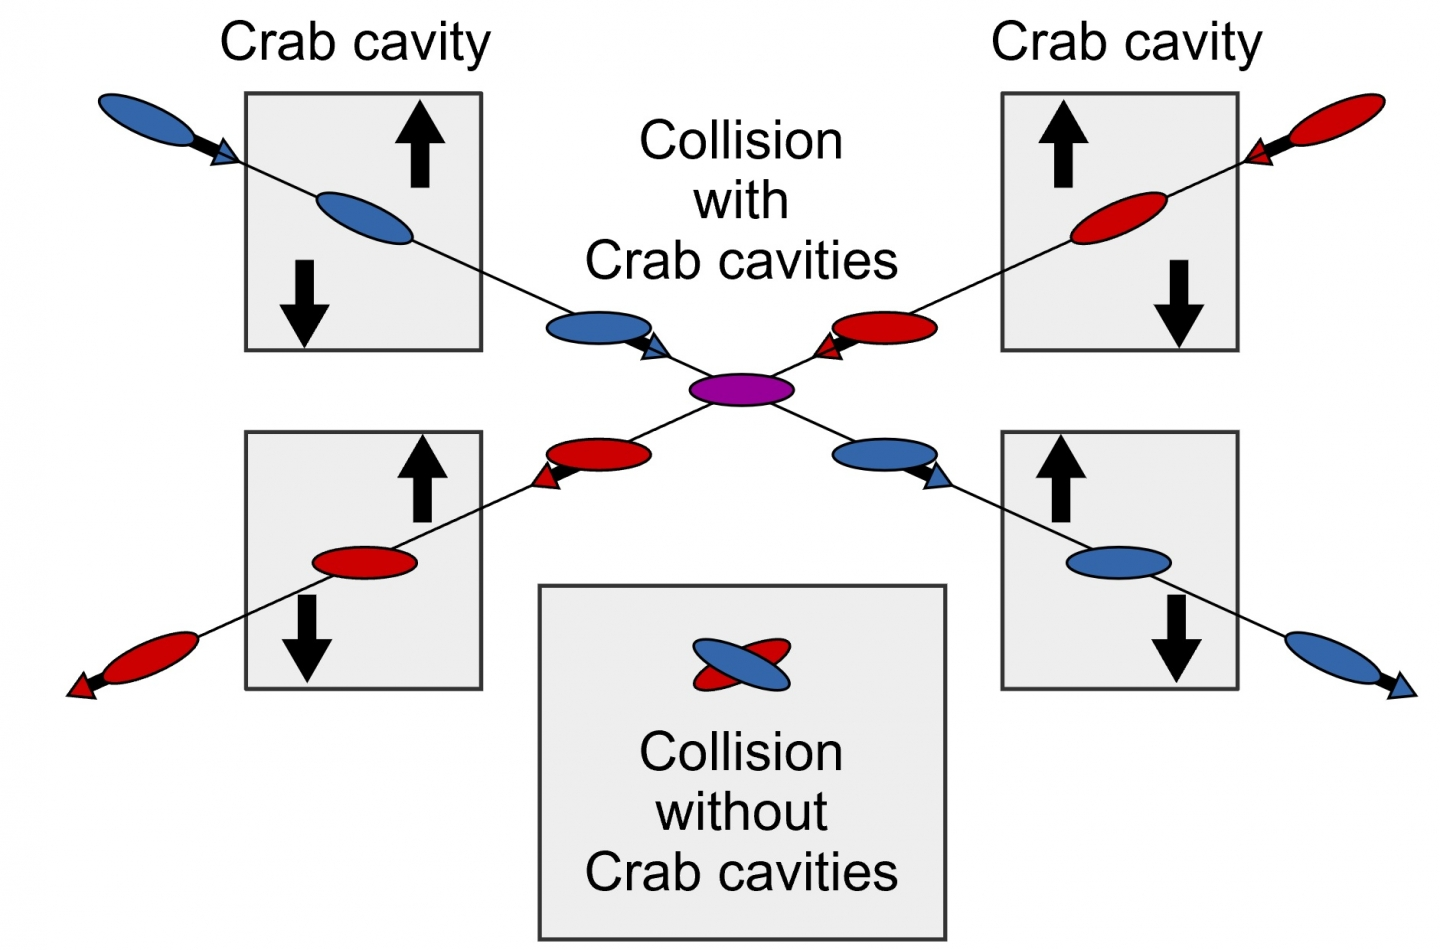
\includegraphics[width=.7\linewidth]{img/crab_cavities.jpg}
    \caption{Crab cavities used to rotate the particle bunches before the collision to maximize the overlap of the colliding bunches. [cite crab-cavities]}
    \label{fig:eic:crab}
\end{figure}

% Compared to HERA, the EIC design implements two new critical ideas:
% \begin{enumerate}
%     \item Flat proton bunches at collisions (to match the electron beam dimensions) - this helps with the
% peak luminosity.
%     \item Continuous proton beam cooling during collisions to maintain matched beam dimensions - this
% helps with the average luminosity.
% \end{enumerate}
% \emph{The SHC-related risk was identified as HIGH.
% To mitigate this risk, we are adding an injection electron cooler for hadrons (at 25 GeV/u) to create ‘flat’ bunches. This is a proven and tested technology. We propose to remove the SHC system from the project baseline.\\}
% [Nagaitsev Frascati]

% from Strong Hadron Cooler to Low Energy Electron Cooler (Ring Electron Cooler - something else?)

% The Ring Electron Cooler must be located in the IR2 of the Hadron Storage Ring (HSR)
